\section{Black Holes}
\label{sec:black-holes}
\subsection{Formation of Black Holes}
A \blackhole{} can form after the gravitational collapse of a sufficiently massive stellar core.

\subsection{Event Horizons}
The event horizon\footnote{The event horizon is a boundary in spacetime beyond which signals cannot reach a distant observer.} is the boundary beyond which light and other signals cannot escape to distant observers.

The Event Horizon Telescope collaboration published an image of the black hole shadow in the galaxy M87 \parencite{eventhorizon2019}.

The \term{event horizon} is an important concept in general relativity.

\begin{figure}[htbp]
    \centering
    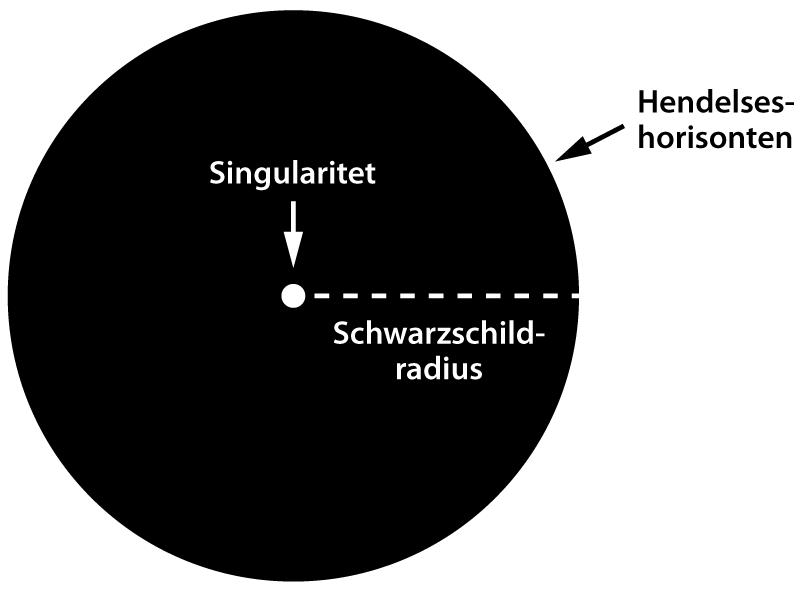
\includegraphics[width=0.75\textwidth]{figures/images/black-hole-diagram.jpg}
    \caption{Simplified schematic of a black hole and its event horizon. Source: Maria Hammerstrøm, SNL (CC BY-NC-SA 3.0). Norwegian labels: singularity, event horizon, Schwarzschild radius.}
    \label{fig:black-hole}
\end{figure}

The Schwarzschild radius is denoted by $r_s$ and depends on the mass $M$ of the object.

The Schwarzschild radius is calculated using Equation~\eqref{eq:schwarzschild-radius}.

\begin{equation}
    r_s = \frac{2GM}{c^2}
    \label{eq:schwarzschild-radius}
\end{equation}